
%(BEGIN_QUESTION)
% Copyright 2015, Tony R. Kuphaldt, released under the Creative Commons Attribution License (v 1.0)
% This means you may do almost anything with this work of mine, so long as you give me proper credit

Suppose a current transformer with a ratio of 400:5 sends its output signal to a protective relay and a panel-mounted ammeter as shown in this schematic diagram:

$$\includegraphics[width=15.5cm]{i02873x01.eps}$$

\begin{itemize}
\item{} $R_{CT}$ = 0.3 $\Omega$ (this is the internal resistance of the CT's secondary winding)
\item{} $R_{wire1}$ = 0.4 $\Omega$
\item{} $R_{wire2}$ = 0.1 $\Omega$
\item{} $R_{wire3}$ = 0.4 $\Omega$
\item{} $R_{relay}$ = 2.5 $\Omega$
\item{} $R_{meter}$ = 1.0 $\Omega$
\end{itemize}

\vskip 10pt

Calculate the following voltage drops in this current transformer circuit, from the given information:

\begin{itemize}
\item{} $V_{relay}$ = \underbar{\hskip 50pt} volts
\vskip 5pt
\item{} $V_{meter}$ = \underbar{\hskip 50pt} volts
\vskip 5pt
\item{} Total voltage dropped across all wires = \underbar{\hskip 50pt} volts 
\vskip 5pt
\item{} Voltage output at CT terminals = \underbar{\hskip 50pt} volts 
\vskip 5pt
\item{} Voltage generated by CT secondary winding (before any $R_{CT}$ losses) = \underbar{\hskip 50pt} volts 
\end{itemize}

\vskip 20pt \vbox{\hrule \hbox{\strut \vrule{} {\bf Suggestions for Socratic discussion} \vrule} \hrule}

\begin{itemize}
\item{} Explain why the two instruments (the relay and the meter) are connected in {\it series} with each other and not in {\it parallel}.
\end{itemize}

\underbar{file i02873}
%(END_QUESTION)





%(BEGIN_ANSWER)

 
%(END_ANSWER)





%(BEGIN_NOTES)

First, we must know how much current is being output by the CT.  With a primary current of 283 amps and a ratio of 400:5, the CT will output:

$$I = \left({283 \hbox{ A} \over 1} \right) \left({5 \over 400} \right) = 3.5375 \hbox{ A}$$

Now that we know the value for $I$, calculating voltage drops is a simple matter of applying Ohm's Law ($V = IR$) to each resistance or collection of series resistances:

$$V_{relay} = I R_{relay} = (3.5375 \hbox{ A})(2.5 \> \Omega) = 8.8438 \hbox{ V}$$

$$V_{meter} = I R_{meter} = (3.5375 \hbox{ A})(1.0 \> \Omega) = 3.5375 \hbox{ V}$$

$$V_{wires} = I (R_{wire1} + R_{wire2} + R_{wire3}) = (3.5375 \hbox{ A})(0.4 \> \Omega + 0.1 \> \Omega + 0.4 \> \Omega) = 3.1838 \hbox{ V}$$

$$V_{CT-terminals} = I (R_{wires} + R_{relay} + R_{meter}) = (3.5375 \hbox{ A})(0.9 \> \Omega + 2.5 \> \Omega + 1.0 \> \Omega) = 15.565 \hbox{ V}$$

$$V_{CT-winding} = I R_{total} = (3.5375 \hbox{ A})(0.9 \> \Omega + 2.5 \> \Omega + 1.0 \> \Omega + 0.3 \> \Omega) = 16.6263 \hbox{ V}$$


%INDEX% Electronics review: current transformer (CT)
%INDEX% Protective relay: CT circuit wire resistance

%(END_NOTES)


